\chapter{Problème}
\section{Solutions de chiffrement possibles LGW <->IN}
Afin de valider si le n\oe{}ud isolé attaché à une LoRaGateway est bien connu de la part de Spot. Il nous faut récupérer les informations afin de réaliser le mode proxy. C'est à dire, MIC, NwkSkey, AppSkey, DevEui, DevNonce, AppNonce, AppKey NetID. Ces informations sont évidemment soumises à plusieurs degrés de sensibilité. Il a été convié que l'AES 128 bits, est une solution assez satisfaisante. Ce qui assure donc une sécurité de bout en bout en AES-128.

\begin{figure}[!ht]    \centering
   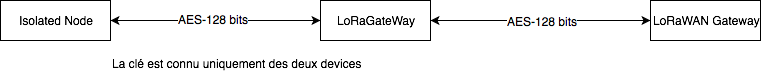
\includegraphics[scale=0.6]{aes-128.png} 
   \caption{Schéma récapitulatif sur le chiffrement}
   \label{Schéma récapitulatif sur le chiffrement}
\end{figure}
Maintenant il y a un choix important à réaliser, en effet l'AES-128 est du chiffrement symétrique. Il est nécessaire de choisir une clé qui doit être connue des deux partis (Device A et B) . \\
Nous avons donc choisi d'utiliser l'échange de clés Diffie-Hellman, qui est une méthode, publiée en 1976, par laquelle deux agents, nommés par convention Alice et Bob, peuvent se mettre d'accord sur un nombre (qu'ils peuvent utiliser comme clé pour chiffrer la conversation suivante) sans qu'un troisième agent appelé Ève puisse découvrir le nombre, même en ayant écouté tous leurs échanges. \\

Voici un déroulement de base tel que nous le concevons lors de la mise en place sur une LoRaGateway et un Isolated node.\\
La LoRaGateway choisit un nombre premier P et une base G. (P et G premier entre eux ). Dans notre exemple, P=23 et G=3\\
la LoRaGateway choisit un nombre secret a=6\\
Elle envoie à Bob la valeur A = $g^a$ [mod P] = $3^6$ [23] = 16\\
Bob choisit à son tour un nombre secret b=15\\
Bob envoie à la LoRaGateway la valeur B = $G^b$ [mod P] = 3\up{15} [23] = 12\\
la LoRaGateway peut maintenant calculer la clé secrète : $B^a$ [mod P] = $12^6$ [23] = 9\\
Bob fait de même et obtient la même clé que la LoRaGateway : $A^b$ [mod P] = 16\up{15} [23] = 9\\

Pour faire simple, La LoRaGateway peut transmettre toutes les données nécessaire en clair c'est à dire P, G, A  à un n\oe{}ud isolé et cela sans aucun soucis. Puisque pour déduire la clé résultante il faut résoudre l'impossibilité (calculatoire) de déduire des seules informations $g^a$, $g^b$, G et P, la valeur de G\up{ab} .
il faut toutefois parler du problème de l'attaque classique du Man in the middle. La parade classique à cette attaque consiste à signer les échanges de valeurs à l'aide d'une paire de clés asymétriques certifiées par une tierce partie fiable, ou dont les moitiés publiques ont été échangées auparavant par les deux participants.

\section{Problème final }
Lors d'un test rapide, la plupart des services qui utilisent l'algorithme de Diffie-Hellman, est gérée par la bibliothèque libre OpenSSL. La force de cet algorithme réside aussi dans les principes mathématiques qu'entourent les nombres premiers, tout comme pour l'algorithme RSA, plus le nombre premier choisi est grand plus la sécurité en est renforcée. Or plus un nombre est grand.. plus il faut s'attendre à gérer des opérations mathématiques très lourdes, en plus de la recherche initiale du nombre premier. Ce qui rappelons le, peut être assez long compte tenu de la puissance de calcul dont dispose un capteur. Ceci n'est que le problème au niveau de la recherche de P. En effet on parle d'une élévation à la puissance (dans la suite du calcul) d'un nombre déjà extrêmement grand, en effet il faut s'attendre à exploser la capacité maximale que peut engranger un nombre en informatique c'est à dire : 18 446 744 073 709 551 615 == 2\up{64}-1 . Pour résoudre ce souci OpenSSL utilise la bibliothèque BIGNUM en C . Qui comme la lib OpenSSL n'est pas disponible sur les capteurs sur lesquels nous développons. 
\section{Conclusion sur le chiffrement}
Il y a plusieurs piste à envisager, celle dont-on parle dans ce document part du principe que nous n'avons aucune autre entrée sécurisée donnée par la LoRaWAN Gateway lors d'un join. La solution à ce problème est probablement du côté des fonctions de type courbes elliptiques comme celles de Diffie-Hellmann . Pour faire simple une solution basée sur les courbes elliptiques serait non implémentable \textbf{sans secure element} . Il est donc nécessaire d'envisager une autre piste. 

